\documentclass[aspectratio=169]{beamer}
\usepackage{import}
\subimport{../../latex/}{setup_presentation}

\title{SYDE 750 Project}
\subtitle{Learning Probability Distributions for Statistical Inference}
\author{Andreas Stöckel}
\date{March 5th, 2017}


\begin{document}

\maketitle

\begin{frame}{Lifespan Inference Task (I)}

Based on \emph{Optimal Predictions in Everyday Cognition} by Griffiths and Tenenbaum (2006)\\[0.5em]

\begin{columns}[t]
	\column{0.5\textwidth}
	\begin{itemize}
		\setlength{\fboxsep}{1pt}
		\item<1-> {\color{violet}Experimental task\textellipsis}\\[0.25em]
		\emph{Insurance agencies employ actuaries to make predictions about people’s lifespans---the age at which they will die---based upon demographic information. If you were assessing an insurance case for an \only<1>{18-year-old}\only<2->{\colorbox{violet}{\color{white}18-year-old}} man, what would you predict for \only<1>{his lifespan}\only<2->{\colorbox{violet}{\color{white}his lifespan}}?}
	\end{itemize}
	\column{0.5\textwidth}
	\begin{itemize}
		\item<2-> {\color{violet}\textellipsis as Bayesian inference}\\[0.25em]
		Given $t$, estimate $t_\mathrm{total}$
		\begin{align*}
			p(t_\mathrm{total} \mid t) = \frac{p(t \mid t_\mathrm{total}) \cdot p(t_\mathrm{total})}{p(t)} \,.
		\end{align*}
		Median estimator, select $\hat t_\mathrm{total}$ s.t.
		\begin{align*}
			p(t_\mathrm{total} > \hat t_\mathrm{total} \mid t) = p(t_\mathrm{total} < \hat t_\mathrm{total} \mid t) \,.
		\end{align*}
	\end{itemize}
\end{columns}
\end{frame}

\begin{frame}{Lifespan Inference Task (II)}

{\centering
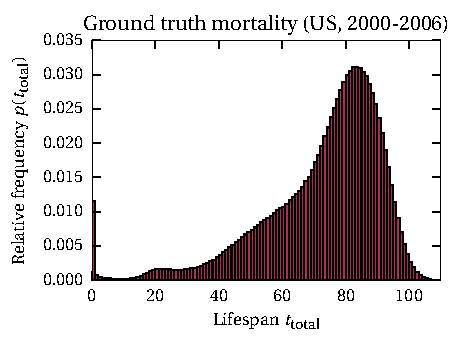
\includegraphics[scale=0.85]{media/mortality_ground_truth.pdf}
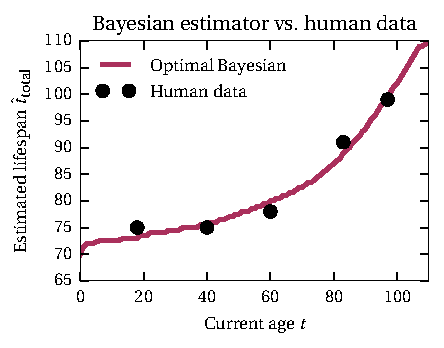
\includegraphics[scale=0.85]{media/mortality_optimal_bayesian_estimator.pdf}}

{\color{gray}\tiny \emph{Mortality data:} Human Mortality Database. University of California, Berkeley (USA), and Max Planck Institute for Demographic Research (Germany). Available at \url{www.mortality.org} (data downloaded on 2017/03/29). \emph{Human experiment results adapted from:} Optimal Predictions in Everyday Cognition. Griffiths and Tenenbaum (2006)}
\end{frame}

\begin{frame}{Outline}
	\begin{itemize}
		\setlength{\itemsep}{0.5em}
		\item {\textcolor{violet}{Motivation}}
		\item {\textcolor{violet}{Part I: Probability Distribution Representation}}\\[0.25em]
		\begin{itemize}
			\setlength{\itemsep}{0.25em}
%			\item Related Work
			\item Non-negative Mixture Model
			\item Implementation
			\item Results
		\end{itemize}
		\item {\textcolor{violet}{Part II: Lifespan Inference}}\\[0.25em]
		\begin{itemize}
			\setlength{\itemsep}{0.25em}
			\item Median Estimation as Gradient Descent
			\item Implementation
			\item Results
		\end{itemize}
		\item {\textcolor{violet}{Conclusion}}
	\end{itemize}
\end{frame}

\begin{frame}
	\centering
	{\Large\textcolor{violet}{\textsc{PART I}}}\\
	\huge Probability Distribution Representation
\end{frame}

% \begin{frame}{Related Work}
% 	TODO
% \end{frame}

\begin{frame}{Non-negative Mixture Model}
\begin{columns}[t]
	\column{0.462\textwidth}
	\begin{block}{Goal}
		Find $p(x)$ which approximates empirical distribution $\mathfrak{P}$. Given samples
		\begin{align*}
			\hat X &= \{ \hat x_1, \ldots, \hat x_N \},\\
			\mathfrak{P}(x \mid \hat X) &= \only<1>{\frac{1}N \cdot} \sum_{i = 1}^N \delta(x - \hat x_i) \,.
		\end{align*}
	\end{block}
	\column{0.462\textwidth}
	\begin{block}{Idea}
		Represent $p(x)$ as non-negative mixture of $k$ basis functions
		\only<1>{\begin{align*}
			p(x) = \frac{\sum_{i = 1}^k w_i \cdot \phi_i(x)} {\sum_{i = 1}^k w_i \cdot \int_{-\infty}^{\infty} \phi_i(x') \, \mathrm{d}x'} \,,
		\end{align*}}
		\only<2>{\begin{align*}
			p(x) = \sum_{i = 1}^k w_i \cdot \phi_i(x) \,,
		\end{align*}}
		where $w_i \geq 0$, $\phi_i(x) \geq 0$\only<1>{, $\int p(x) \,\mathrm{d}x = 1$}.
	\end{block}
\end{columns}
\begin{overlayarea}{\textwidth}{2cm}
	\vspace{1cm}
	\centering
	\only<2->{\large\textcolor{violet}{Ignore Normalization! {\symbolfont 🐉}}}
\end{overlayarea}
\end{frame}

\begin{frame}{Learning Probability Distributions}
	\begin{columns}[t]
		\column{0.462\textwidth}
		\begin{block}<1->{Batch Learning}
			\begin{itemize}
				\setlength{\itemsep}{1em}
				\item<2-> Given $\hat X$ find $\vec w$ s.t.
					$$p(x \mid \vec w) \approx \mathfrak{P}(x \mid \hat X)$$
				\item<3-> Expectation Maximization!
				\item<4-> Nope, really just $L_2$ regression\\(nonparametric $\phi_i$, single $E$-step)
			\end{itemize}
		\end{block}
		\column{0.462\textwidth}
		\begin{block}<5->{Online Learning}
			\begin{itemize}
				\setlength{\itemsep}{1em}
				\item<5-> For each sample $\hat x_i$ find new $\vec w'$ s.t.
					$$p(x \mid \vec w') \approx p(x \mid \vec w) + \delta(x - \hat x_i)$$
				\item<6-> Online Expectation Maximization!
				\item<7-> Again, way too complex...
			\end{itemize}
		\end{block}
	\end{columns}
\end{frame}

\begin{frame}{Learning Probability Distributions -- Optimal online update rule}
	\begin{overlayarea}{\textwidth}{0.8\textheight}
	For each new sample $\hat x$ minimize quadratic approximation error w.r.t. $\Delta w_j = w_j' - w_j$:
	\begin{align*}
	\only<1->{\frac{\mathrm{\partial}}{\mathrm{\partial}\Delta w_j} \; E &=
	\frac{\mathrm{\partial}}{\mathrm{\partial}\Delta w_j} \; \int_{-\infty}^\infty \frac{1}2
		\left(
			p(x \mid \vec w') - p(x \mid \vec w) - \delta(x - \hat x) 
		\right)^2 \;\mathrm{d}x} \\
	\only<2->{&= \frac{\mathrm{\partial}}{\mathrm{\partial}\Delta w_j} \; \int_{-\infty}^\infty \frac{1}2
		\left(
			\sum_{i=1}^k \Delta w_i \cdot \phi_i(x) - \delta(x - \hat x) 
		\right)^2 \;\mathrm{d}x} \\
	\only<3->{&= \int_{-\infty}^\infty
			\sum_{i=1}^k \Delta w_i \cdot \phi_j(x) \cdot \phi_i(x) - \phi_j(x) \cdot \delta(x - \hat x) 
		\;\mathrm{d}x} \\
	\only<4->{&= \sum_{i=1}^k \Delta w_i \cdot \underbrace{\int_{-\infty}^\infty \phi_j(x) \cdot \phi_i(x) \;\mathrm{d}x}_{\gamma_{ij}} - \phi_j(\hat x) \overset{!} = 0} \\
	\only<5->{\Leftrightarrow \Delta \vec w
	&= \Gamma^{-1} \cdot \vec \phi(\hat x)} \only<6->{\color{violet} \Rightarrow \Delta \vec w \text{ linear combination of } \vec \phi(\hat x) \text{!}} \only<7->{\text{\symbolfont 🐇}}
	\end{align*}
	\end{overlayarea}
\end{frame}

\begin{frame}{Basis Functions -- Radial basis}

\centering

Radial basis function $\phi_i(x) = \phi\left(\frac{\| x - x_i \|}{\sigma}\right)$

\vspace{0.5cm}

{\color{violet}\hspace{1cm}Box basis\hspace{1.9cm}Cosine basis\hspace{1.6cm}Gaussian basis}\\
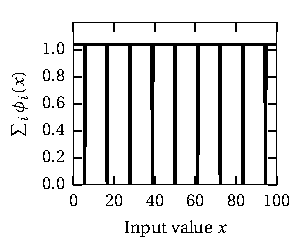
\includegraphics[scale=0.85]{../media/basis_box.pdf}
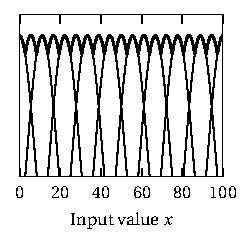
\includegraphics[scale=0.85]{../media/basis_cosine.pdf}
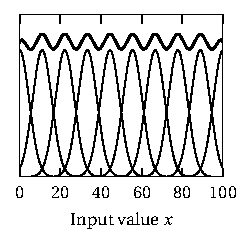
\includegraphics[scale=0.85]{../media/basis_gaussian.pdf}

\begin{align*}
	  \phi^\mathrm{box}(r) &= \begin{cases}
				1 & \text{if } r \leq 1 \\
				0 & \text{if } r > 1
	           \end{cases},
	& \phi^\mathrm{cos}(r) &= \begin{cases}
	              \cos(r) & \text{if } r \leq \frac{\pi}2 \\
	              0       & \text{if } r > \frac{\pi}2 \\
	             \end{cases},
	& \phi^\mathrm{gauss}(r) &= \exp\left(-r^2\right)
\end{align*}

\end{frame}

\begin{frame}{Basis Functions -- How to select $\sigma$?}

Radial basis function $\phi_i(x) = \phi\left(\frac{\| x - x_i \|}{\sigma}\right)$

Matrix of inner products $(\Gamma)_{ij} = \gamma_{ij} = \int_{-\infty}^\infty \phi_j(x) \cdot \phi_i(x) \;\mathrm{d}x$

\begin{columns}[t]
	\column{0.4\textwidth}
	\begin{block}<1->{Two constraints}
	\begin{itemize}
		\item<1-> Near-orthogonal basis
			$$\Gamma = I = \Gamma^{-1} \Rightarrow \Delta \vec w = \vec \phi(\hat x)$$
		\item<2-> Constant support
			$$\sum_{i = 1}^k \phi_i(x) - \phi_i(y) \approx 0 \, \forall x, y$$
	\end{itemize}
	\end{block}
	\column{0.5\textwidth}
	\begin{block}<3->{Heuristic}
		Numerically minimize w.r.t. $\sigma$
		\begin{align*}
		E(\sigma) &= \left(1 - \min_x(f(x; \sigma))\right)^2 \\
		&+ \left(1 - \max_x(f(x; \sigma))\right)^2 \\
		&\, \text{where } f(x; \sigma) = \sum_{i = 1}^k \phi_i(x)
		\end{align*}
	\end{block}
\end{columns}

\end{frame}

\begin{frame}{Basis Functions -- $\Gamma$ matrices}
\centering
{\hspace{1cm}Box basis\hspace{2.25cm}Cosine basis\hspace{2cm}Gaussian basis}\\
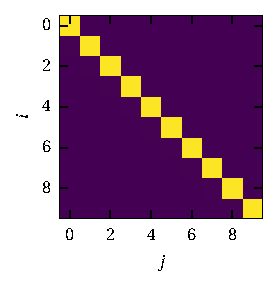
\includegraphics[scale=0.85]{../media/basis_box_prod.pdf}
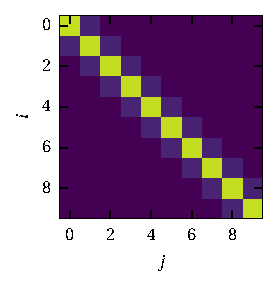
\includegraphics[scale=0.85]{../media/basis_cosine_prod.pdf}
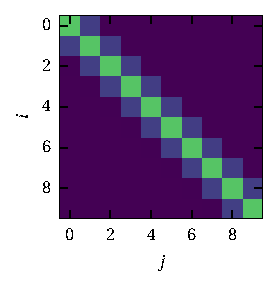
\includegraphics[scale=0.85]{../media/basis_gaussian_prod.pdf}\\
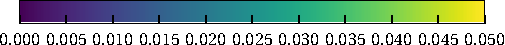
\includegraphics[scale=0.85]{../media/inner_prod_cbar.pdf}\\[0.25cm]

After thorough visual inspection we conclude
\begin{align*}
\Gamma \approx I
\end{align*}
\end{frame}

\begin{frame}{Probability Distribution Network Implementation (I)}
	\centering
	Implementation of $p(x) = \sum_{i = 1}^k w_i \cdot \phi_i(x)$ as a neural network\\[0.5cm]
	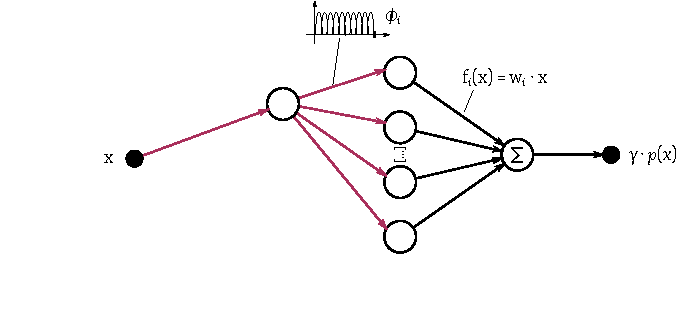
\includegraphics{media/network_diagram_01.pdf}
\end{frame}

\begin{frame}{Learning Rule}
	\begin{block}{Idea}
		Use Prescribed Error Sensitivity (PES) rule to learn functions $f_i$
	\end{block}
	\vspace{0.5cm}
	\begin{block}{Derivation}
		\begin{columns}[t]
			\column{0.462\textwidth}
			\begin{itemize}
				\item {\color{violet}\emph{Assumption:}}\\
					Current function $f_i(x) = w_i \cdot x$
			\end{itemize}
			\column{0.462\textwidth}
			\begin{itemize}
				\item {\color{violet}\emph{Desired:}}\\
					Updated function $f'_i(x) = w_i' \cdot x$
			\end{itemize}
		\end{columns}
		\begin{overlayarea}{\textwidth}{2.75cm}
		\begin{align*}
			\only<2->{E_i &= f_i(\phi_i(x)) - f_i'(\phi_i(x)) \hspace{5.75cm}} \\
			\only<3->{&= w_i \cdot \phi_i(x) - w'_i \cdot \phi_i(x)
				 = -\Delta w_i \cdot \phi_i(x)} \\
			\only<4->{&= - (\Gamma^{-1} \cdot \vec \phi(x))_i \cdot \phi_i(x)
				 \approx - (I \cdot \vec \phi(x))_i \cdot \phi_i(x)
				 = -\phi_i(x)^2}
		\end{align*}
		\end{overlayarea}
	\end{block}
\end{frame}

\begin{frame}{Probability Distribution Network Implementation (II)}
	\begin{overlayarea}{\textwidth}{0.8\textheight}
	\centering
	Implementation of $p(x) = \sum_{i = 1}^k w_i \cdot \phi_i(x)$ as a neural network\\[0.5cm]
	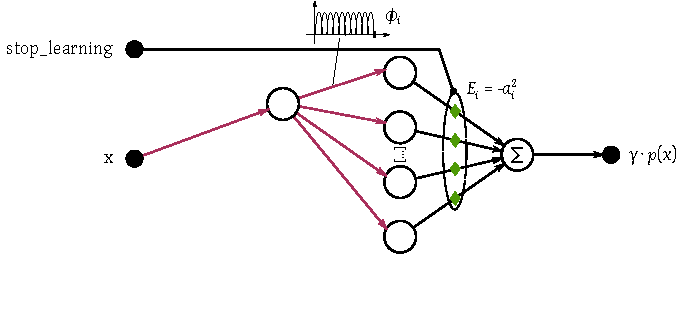
\includegraphics{media/network_diagram_02.pdf}\\
	\only<2->{{\color{violet}\emph{Important:}} Select tuning curves for $E_i$ populations such that $\vec a_i = 0 \Leftrightarrow E_i = 0$}
	\end{overlayarea}
\end{frame}

\begin{frame}{Experimental results (I)}
\begin{overlayarea}{\textwidth}{0.85\textheight}
\centering
{\small\hspace{0.45cm}\only<1>{Box basis}\only<2>{Cosine basis}\only<3>{Gaussian basis}}\\%
\only<1>{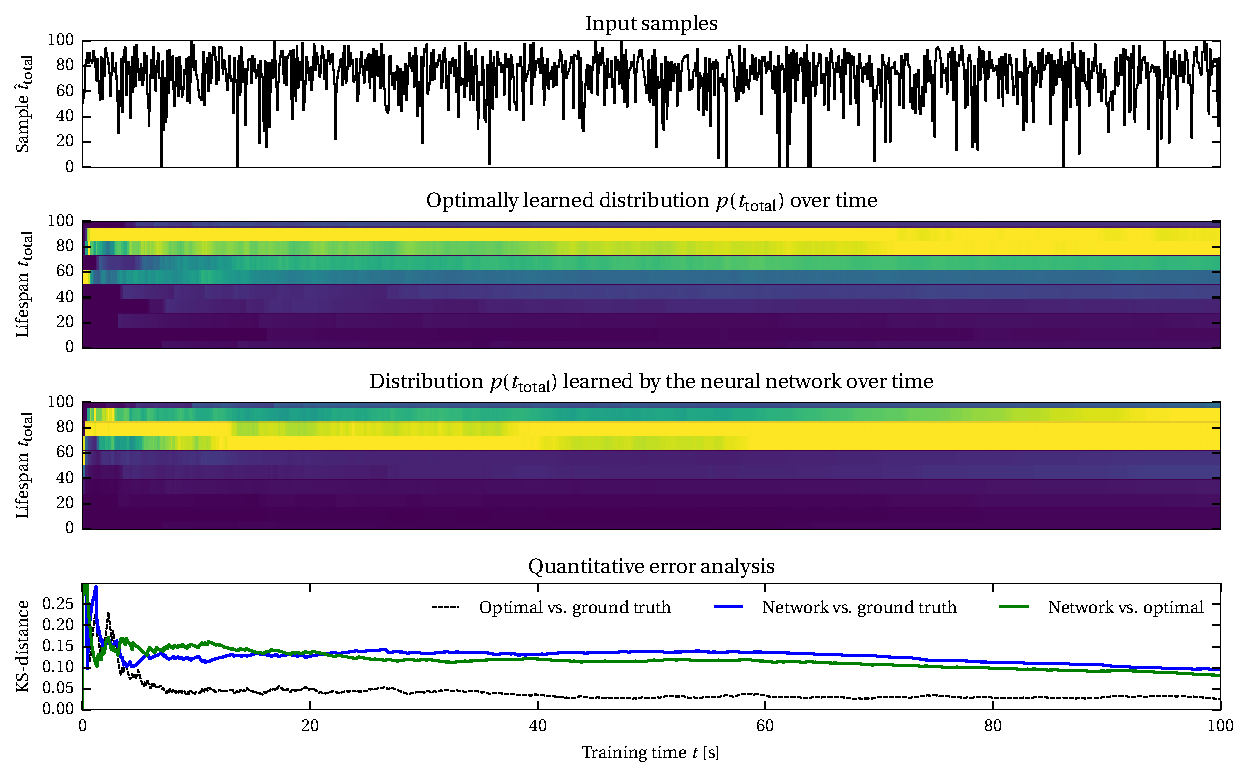
\includegraphics[width=0.85\textwidth]{../media/net_probability_box_10_100000_0.pdf}}%
\only<2>{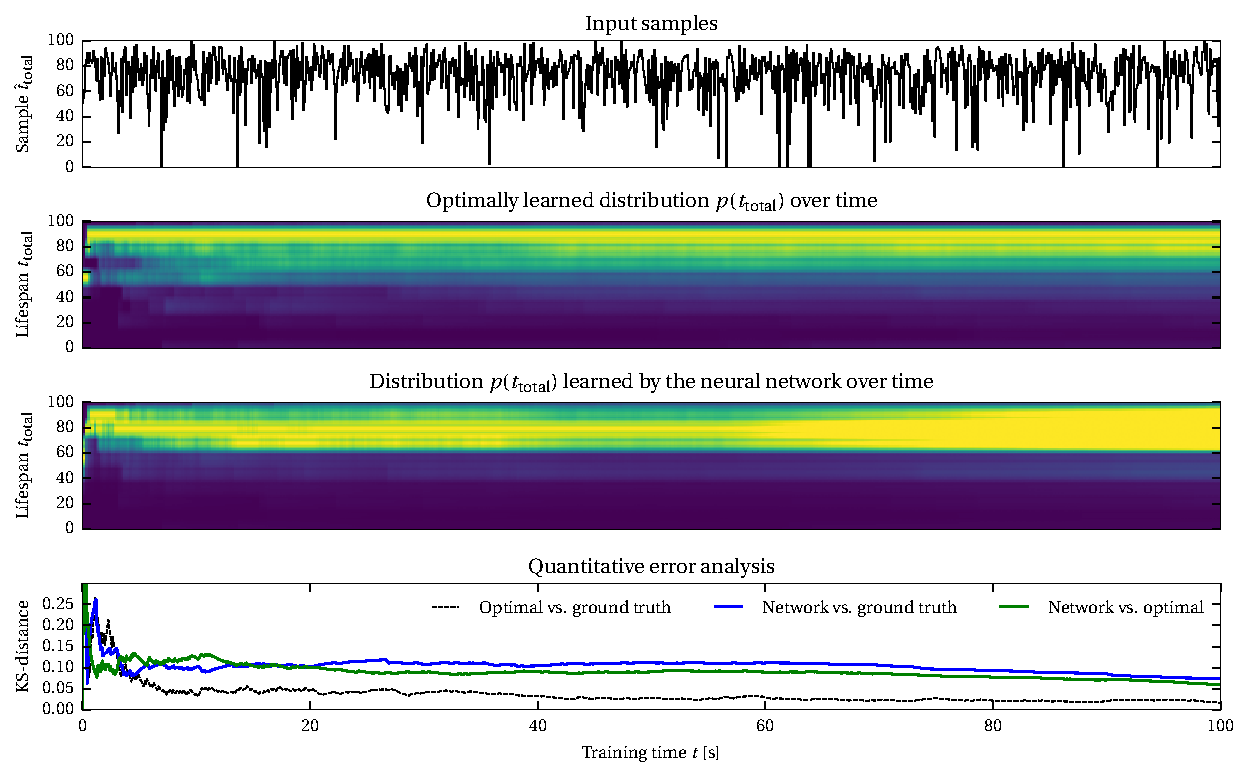
\includegraphics[width=0.85\textwidth]{../media/net_probability_cosine_10_100000_0.pdf}}%
\only<3>{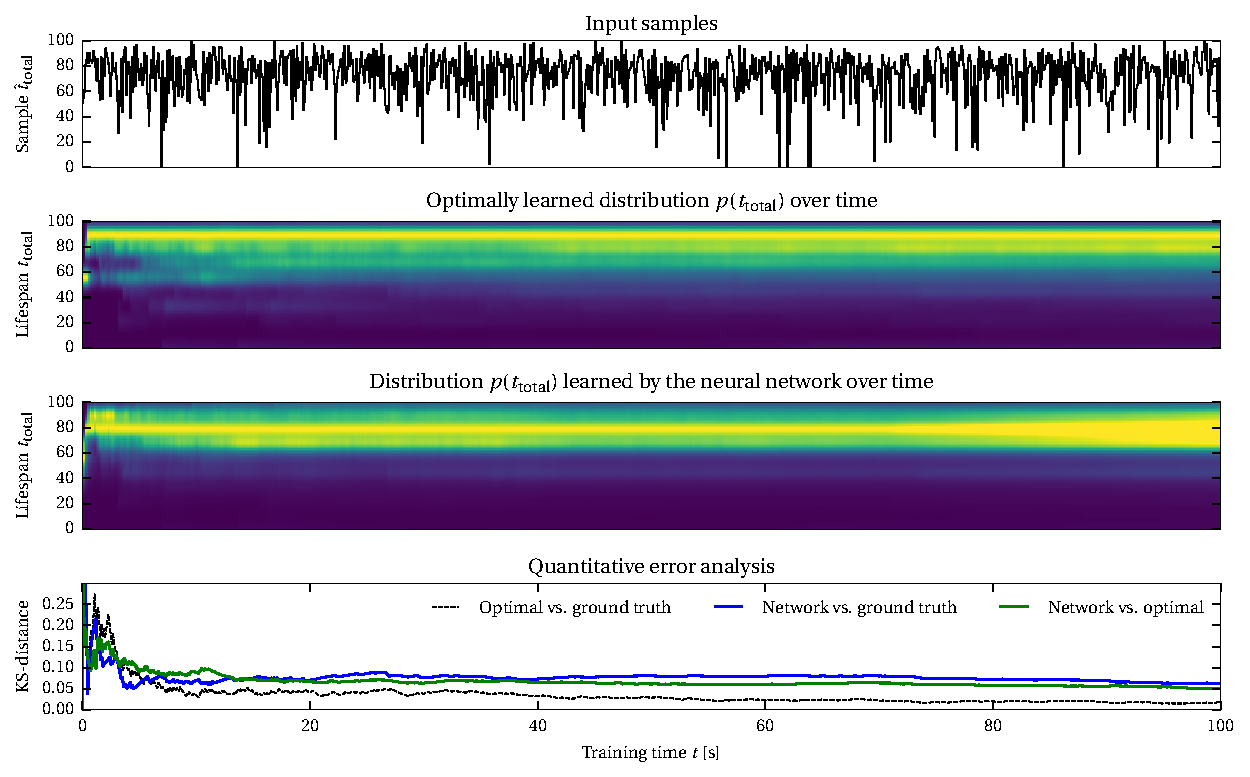
\includegraphics[width=0.85\textwidth]{../media/net_probability_gaussian_10_100000_0.pdf}}%
\end{overlayarea}
\end{frame}

\begin{frame}{Experimental results (II)}

\centering
{\color{violet}\hspace{1cm}Box basis\hspace{2cm}Cosine basis\hspace{1.75cm}Gaussian basis}\\
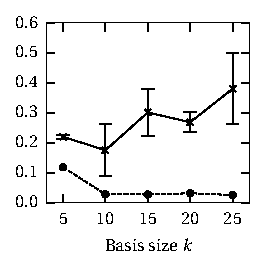
\includegraphics[scale=0.85]{../media/net_probability_box_errs.pdf}
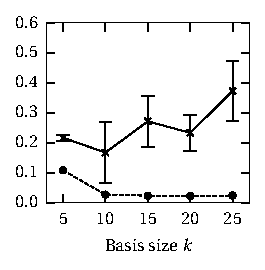
\includegraphics[scale=0.85]{../media/net_probability_cosine_errs.pdf}
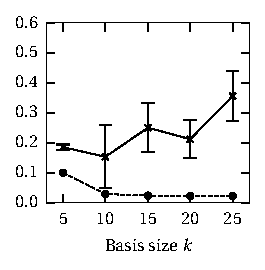
\includegraphics[scale=0.85]{../media/net_probability_gaussian_errs.pdf}\\[0.25cm]

\footnotesize
\centering
{\color{violet}\emph{Dashed line:}} optimal vs. ground truth.
{\color{violet}\emph{Solid line:}} learned vs. ground truth.\\[0.25cm]
Errors expressed in a two-sample Kolmogorov-Smirnov metric.\\
Mean, standard deviation over $N = 5$ trials.
\end{frame}

\begin{frame}{Part I -- Summary}
	\begin{block}<1->{What I've shown you so far\textellipsis}
	\begin{itemize}
		\item We are able to represent a prior probability distribution $p(t_\mathrm{total})$.
		\item Distribution implicitly stored as a weight vector $\vec w$ in the connections between neuron ensembles.
		\item Learning of $\vec w$ using a local PES rule.
	\end{itemize}
	\end{block}
	\begin{block}<2->{What is missing?}
	\begin{itemize}
		\item Representation of the posterior $p(t_\mathrm{total} \mid t)$.
		\item Median estimation.
	\end{itemize}
	\end{block}	
\end{frame}

\begin{frame}
	\centering
	{\Large\textcolor{violet}{\textsc{PART II}}}\\
	\huge Lifespan Inference
\end{frame}

\begin{frame}{Basis function transformation (I)}
\begin{columns}[T]
	\column{0.462\textwidth}
	\begin{block}{Probability distribution $p(x)$}
	\begin{align*}
		p(x) = \sum_{i = 1}^k w_i \cdot \phi_i(x)
	\end{align*}
	\end{block}
	\column{0.462\textwidth}
	\centering
	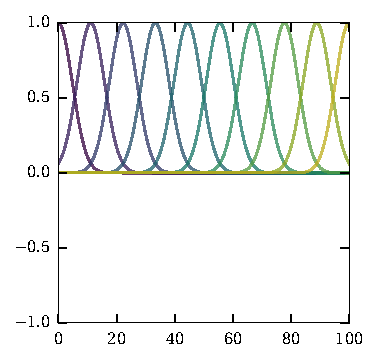
\includegraphics[width=\textwidth]{media/basis_gaussian_distr.pdf}\\
	\footnotesize Basis functions $\phi_i(x)$
\end{columns}
\end{frame}

\begin{frame}{Basis function transformation (I)}
\begin{columns}[T]
	\column{0.462\textwidth}
	\begin{block}{Cumulative distribution $p(x \leq x')$}
	\begin{align*}
		p(x \leq x')
			&= \int_{-\infty}^{x'} \sum_{i = 1}^k w_i \cdot \phi_i(x) \,\mathrm{d}x\\ 
			&= \sum_{i = 1}^k w_i \cdot \int_{-\infty}^{x'} \phi_i(x) \,\mathrm{d}x\\
			&= \sum_{i = 1}^k w_i \cdot \Phi'_i(x')
	\end{align*}
	\end{block}
	\column{0.462\textwidth}
	\centering
	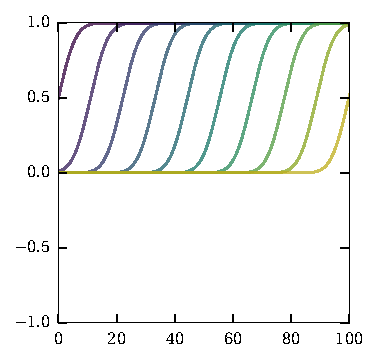
\includegraphics[width=\textwidth]{media/basis_gaussian_cum.pdf}\\
	\footnotesize Basis functions $\Phi'_i(x)$
\end{columns}
\end{frame}

\begin{frame}{The Median Gradient}

\begin{block}{Idea}
\begin{itemize}
	\item<1-> Per definition $g(x') = p(x \leq x') - p(x \geq x') = 0 \Leftrightarrow x'$ is the median of $p(x)$.
%	\item<2-> $g(x')$ is monotonic!
	\item<2->[$\Rightarrow$] Dynamical system $\frac{\mathrm{d}}{\mathrm{d}t} x' = -g(x')$ converges to the median over time $t$!
	\item<3-> {\color{violet}\emph{Note:}} In contrast to $p(x) = 0.5$ above median definition invariant to normalization.
\end{itemize}
\end{block}

\begin{block}<5->{Basis transformation}
\begin{align*}
	p(x \leq x') - p(x \geq x')
		&= \int_{-\infty}^{x'} \sum_{i = 1}^k w_i \cdot \phi_i(x) \,\mathrm{d}x
			- \int_{x'}^{\infty}  \sum_{i = 1}^k w_i \cdot \phi_i(x) \,\mathrm{d}x\\ 
		&= \sum_{i = 1}^k w_i \cdot \left(
				\int_{-\infty}^{x'} \phi_i(x) \,\mathrm{d}x
			- \int_{x'}^{\infty}  \phi_i(x) \,\mathrm{d}x \right)
			= \sum_{i = 1}^k w_i \cdot \Phi_i(x')
\end{align*}
\end{block}

\end{frame}

\begin{frame}{Basis function transformation (II)}
\begin{columns}[T]
	\column{0.462\textwidth}
	\begin{overlayarea}{\textwidth}{6cm}
	\begin{block}{Median gradient $g(x')$}
	\begin{align*}
		p(x \leq x') - p(x \geq x')
			&= \sum_{i = 1}^k w_i \cdot \Phi_i(x')
	\end{align*}
	\begin{itemize}
		\item<2->[$\Rightarrow$] We can calculate the median gradient \emph{without} changing the learned $\vec w$.
		\item<3->[$\Rightarrow$] Just change the decoded function.
	\end{itemize}
	\end{block}
	\end{overlayarea}
	\column{0.462\textwidth}
	\centering
	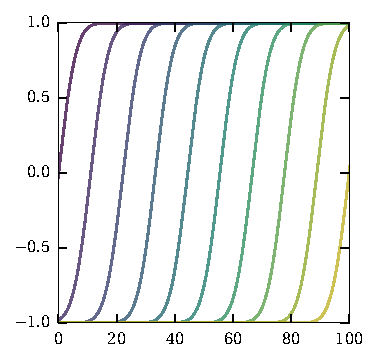
\includegraphics[width=\textwidth]{media/basis_gaussian_median.pdf}\\
	\footnotesize Basis functions $\Phi_i(x)$
\end{columns}
\end{frame}

\begin{frame}{Probability distribution representation and median estimation network}
	\centering
	Implementation of $p(x \leq x') - p(x \geq x') = \sum_{i = 1}^k w_i \cdot \Phi_i(x)$ as a neural network\\[0.5cm]
	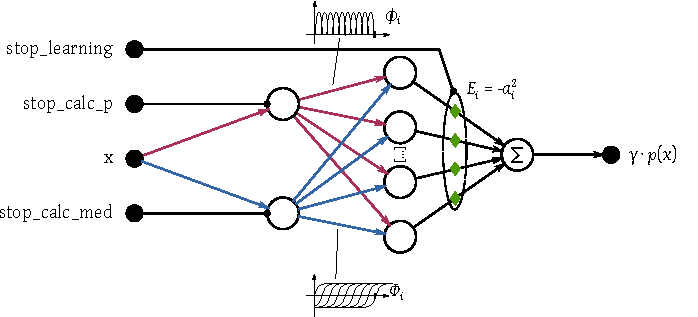
\includegraphics{media/network_diagram_04.pdf}
\end{frame}

\begin{frame}{Inference}
	\begin{itemize}
		\item {\color{violet}\emph{Goal}:}\\
		Calculate median of the posterior distribution
		\begin{align*}
			P(t_\mathrm{total} \mid t)
				\propto P(t \mid t_\mathrm{total}) \cdot P(t_\mathrm{total})
				= \begin{cases}
				    \frac{P(t_\mathrm{total})}{t_\mathrm{total}} & \text{if } t < t_\mathrm{total} \\
				    0 & \text{otherwise}
				   \end{cases}
		\end{align*}
		\item {\color{violet}\emph{Basis functions $\Phi_i(x, y)$}:}\\
		\begin{align*}
			\Phi_i(x, y) =
				\int_{-\infty}^{\hat{x}}
					p(y \mid x') \cdot \phi_i(x') \; \mathrm{d}x' -
				\int_{\hat{x}}^{\infty}
					p(y \mid x') \cdot \phi_i(x') \; \mathrm{d}x'
		\end{align*}
	\end{itemize}
\end{frame}


\begin{frame}{Wait! There is a problem!}
	\begin{block}<2->{Learned $f(x) = w_i \cdot x$ is not defined over negative $x$!}
		\begin{itemize}
			\setlength{\itemsep}{0.5cm}
			\item<3-> PES rule: $\Delta \vec d_i = \kappa \cdot E \cdot \vec a_i$
			\item<4-> Basis functions $\phi_i(x)$ are non-negative\\
			{\color{violet}$\Rightarrow$} activation $\vec a_i$ never represents negative values!
			\item<5-> {\color{violet}\emph{But:}} basis functions $\Phi_i(x, y)$ are defined over $[-1, 1]$!
		\end{itemize}
	\end{block}
	\begin{block}<6->{Solution}
		\begin{itemize}
		\item[$\Rightarrow$] Two symmetric probability distribution networks representing the positive and negative branch of $\Phi(x, y)$
		\end{itemize}
	\end{block}
\end{frame}

\begin{frame}{Lifespan Inference Network Overview}
	\begin{columns}
		\column{0.5\textwidth}
		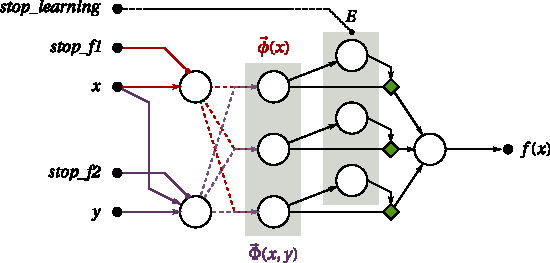
\includegraphics[width=\textwidth]{../media/diag_px.pdf}
		\column{0.5\textwidth}
		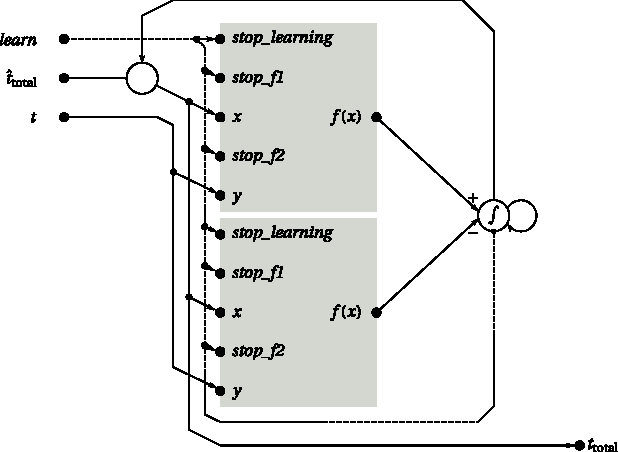
\includegraphics[width=\textwidth]{../media/diag_overall.pdf}%
	\end{columns}
	\centering
	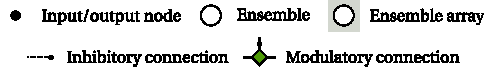
\includegraphics[scale=0.7]{../media/diag_legend.pdf}
\end{frame}

\begin{frame}{Lifespan Inference Results}
	\centering
	\includegraphics<1>[width=0.9\textwidth]{../media/net_lifespan_gaussian_10_const_0.pdf}
	\includegraphics<2>[width=0.9\textwidth]{../media/net_lifespan_gaussian_10_t_0.pdf}
	\includegraphics<3>[width=0.7\textwidth]{../media/net_lifespan_analysis_legend.pdf}\\[0.25cm]
	\includegraphics<3>[width=0.5\textwidth]{../media/net_lifespan_gaussian_10_const_analysis.pdf}
	\includegraphics<3>[width=0.5\textwidth]{../media/net_lifespan_gaussian_10_t_analysis.pdf}
	\only<3>{\\\hspace{0.5cm}{\color{violet}\emph{(a)}} Constant $\hat t^\mathrm{total}$ \hspace{4.5cm}
	{\color{violet}\emph{(b)}} $\hat t^\mathrm{total} = t$}
\end{frame}

\begin{frame}{Conclusion}
	\begin{block}{Results}
		\begin{itemize}
			\setlength{\itemsep}{0.25cm}
			\item Network capable of learning the prior distribution $p(t_\mathrm{total})$.
			\item Lifespan inference not perfect, but shows the right qualitative behaviour.
		\end{itemize}
	\end{block}
	\begin{block}{Questions}
		\begin{itemize}
			\setlength{\itemsep}{0.25cm}
			\item Switching decoders by inhibiting populations an interesting computational principle?
			\item Statistical inference as gradient descent plausible?
			\item Derivation for $E_i = -a_i^2$ might not be correct (dynamics of the PES rule).
			\item Learning rule for linear functions which does not require symmetric populations?
			\item Some way to normalize weights, e.g.~$\|\vec w\| = 1$?
		\end{itemize}
	\end{block}
\end{frame}


\begingroup
\setbeamercolor{background canvas}{bg=black}
\begin{frame}
	\centering
	\color{white}
	\vspace{0.5cm}
	{\huge Thank you for your attention!\\\normalsize Questions? Comments?}\\[0.25cm]
\end{frame}
\endgroup

\end{document}
